\documentclass[../thesis.tex]{subfiles}
% Separate preamble for this subfile. This preamble is loaded last, so one can override various functions before \begin{document}

% Better comment extension for Vscode colors these comments differently
% Normal comment color
% * Important information
% ! ALERT
% ? Question
% TODO stuff to do
% // This is strikethrough


\begin{document}
However interesting the Penrose and Escher tilings appear, we will only focus on monohedral tilings of $\R^d$ by translation, using the unit cube as our tile. Considering only cube-tilings might seem simple initially, but we will see that as we increase the dimension, we get increased flexibility and more complex tilings. It turns out that in higher dimensions, highly exotic and counterintuitive cube tilings exist. The fact that this kind of tiling exists in the first place is surprising in light of Keller's \namecref{thrm:keller_tiling} \cite{iosevichSpectralTilingProperties1998}.

%\begin{theorem}  %* (My original) Keller theorem from the paper of Iosovich and Pedersen
%    Given a discrete subset $T\subset \R^d$. If $T$ is a tiling set for $\Omega$, then given any pair $\lambda, \lambda' \in T$ such that $\lambda\neq\lambda'$, there exists a $j\in \braq{1,\dots,d}$ so that $\bral{t_j -t_j' } \in \N$
%\end{theorem}
%\begin{theorem}  %* Keller theorem from the paper of Lagarias and Reeds
%    If $\Lambda + \bras{0,1}^n$ is a tiling of $\R^n$, then each $\lambda,\lambda'\in \Lambda$ has
%    \begin{equation*}
%        \lambda_i - \lambda_i' \in \intnozero \quad \text{ for some } i, \quad 1\leq i \leq n.
%    \end{equation*}
%\end{theorem}
\begin{theorem}[Keller's theorem]\label{thrm:keller_tiling}
    %Let $\Lambda \subset \R^d$ be a discrete subset.  %* No need to specify, as we will define the tiling set later
    If $\Lambda$ is a tiling set for the unit cube, then for any two $\lambda, \lambda' \in \Lambda$ with $\lambda\neq\lambda'$, there exist a $j\in \braq{1,\dots,d}$ so that $\lambda_j-\lambda_j' \in \intnozero$.
\end{theorem}

We will formally define what we mean by a \emph{tiling set} from \cref{thrm:keller_tiling} later (\cref{def:tiling}), but for now, we continue this informal discussion on exotic tilings. Keller's \namecref{thrm:keller_tiling} is one of the main aims of the \namecref{chap:tiling} and will later be proven in \cref{sec:proof_keller}. Equally important is that Keller also conjectured the following in the same paper \cite{kellerUberLuckenloseErfullung1930} where \cref{thrm:keller_tiling} was first stated and proven. 

\begin{conjecture}[Keller's \namecref{conj:keller_tiling}]\label{conj:keller_tiling}
    All tilings of $\R^d$ by translations of the unit cube contain \textsc{two} cubes that share an entire $(d-1)$-dimensional face.
\end{conjecture}  %* For å kaste lys på at de kan være eksotiske så er det det at de er usant over 7 som er det relevante her. 


% fill=gray!50

\begin{figure}[t!]%h!
    \centering
    \begin{subfigure}{.47\textwidth}
        \centering
        %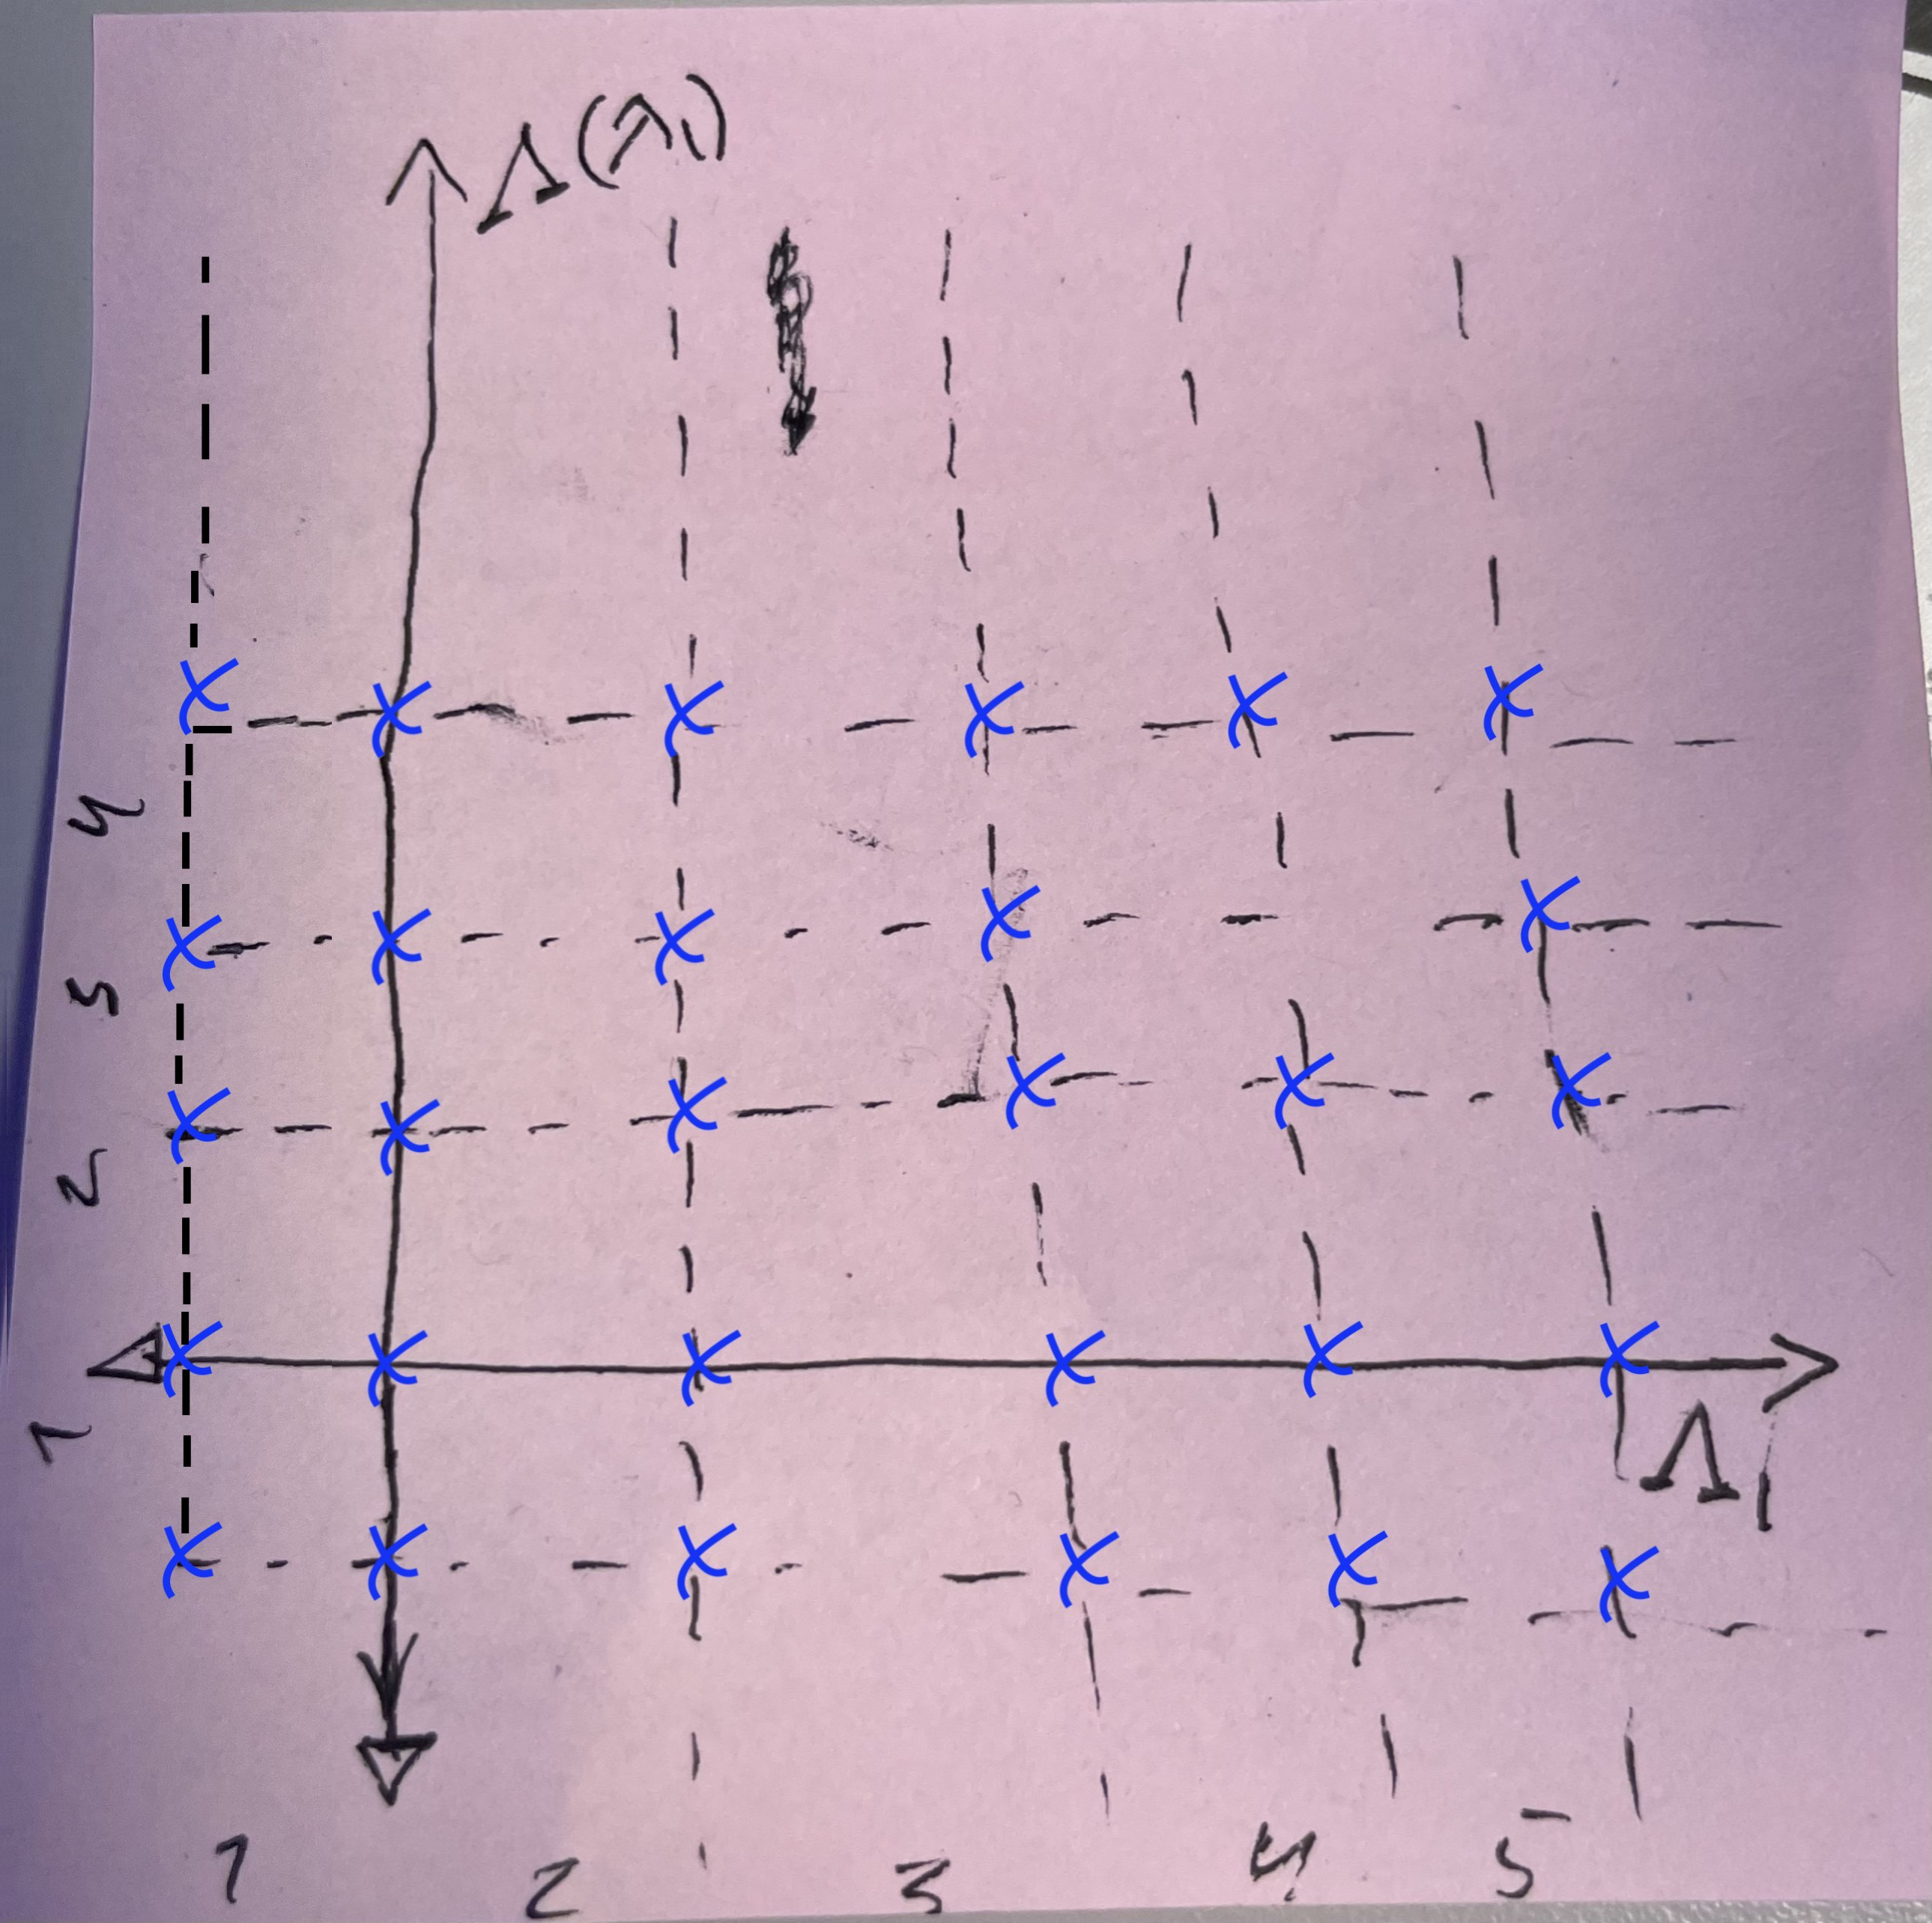
\includegraphics[width=0.9\linewidth]{spec_no_shift.jpg}
        %* Figure 1
        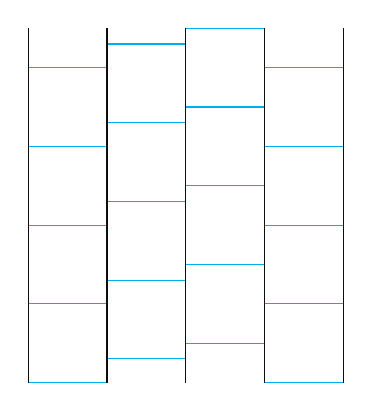
\begin{tikzpicture}[scale=1]
            % Define the tile
            \def\tile{
            %\draw (1,0) -- (1,1) -- (0,1) -- (0,0) -- cycle;  % Draw the unit square
            \draw[black!95] (0,0) rectangle (1,1);
            %\draw (0,0) rectangle (1,1);
            \draw[cyan] (0,0) -- (1,0);
            \draw[cyan] (0,1) -- (1,1);
            }
            
            % Draw the tiling pattern
            \foreach \x in {0,1,2,3}{
                \foreach \y in {0,1,2,3}{
                    % Here we shift with different z values for each height value 
                    % i.e. Row shift
                    \ifnum\x=0
                        \pgfmathsetmacro{\shiftX}{\x} % Set horizontal shift
                        \pgfmathsetmacro{\shiftY}{\y}
                    \fi
                    \ifnum\x=1
                        \pgfmathsetmacro{\shiftX}{\x} % Set horizontal shift
                        \pgfmathsetmacro{\shiftY}{\y+0.3}
                    \fi
                    \ifnum\x=2
                        \pgfmathsetmacro{\shiftX}{\x} % Set horizontal shift
                        \pgfmathsetmacro{\shiftY}{\y+0.5}
                    \fi
                    \ifnum\x=3
                        \pgfmathsetmacro{\shiftX}{\x} % Set horizontal shift
                        \pgfmathsetmacro{\shiftY}{\y}
                    \fi
                    \begin{scope}[shift={(\shiftX,\shiftY)}]
                        \tile % Draw the tile
                    \end{scope}
                }
            }
            % black lines to hide the blue lines
            \foreach \x in {0,1,2,3,4}{
                \draw[ black!95] (\x,0) -- (\x,4);
                \draw[black!95] (\x,0+0.3) -- (\x,4+0.3);
                \draw[black!95] (\x,0+0.3) -- (\x,4+0.5);
                \draw[black!95] (\x,0) -- (\x,4+0.5);
                \draw[black!95] (\x,0) -- (\x,4);
            }
        \end{tikzpicture}
        %* —————————————————
        %\caption{Lattice tiling}
        \label{fig:tiling_five}
    \end{subfigure}\quad
    \begin{subfigure}{.47\textwidth}
        \centering
        %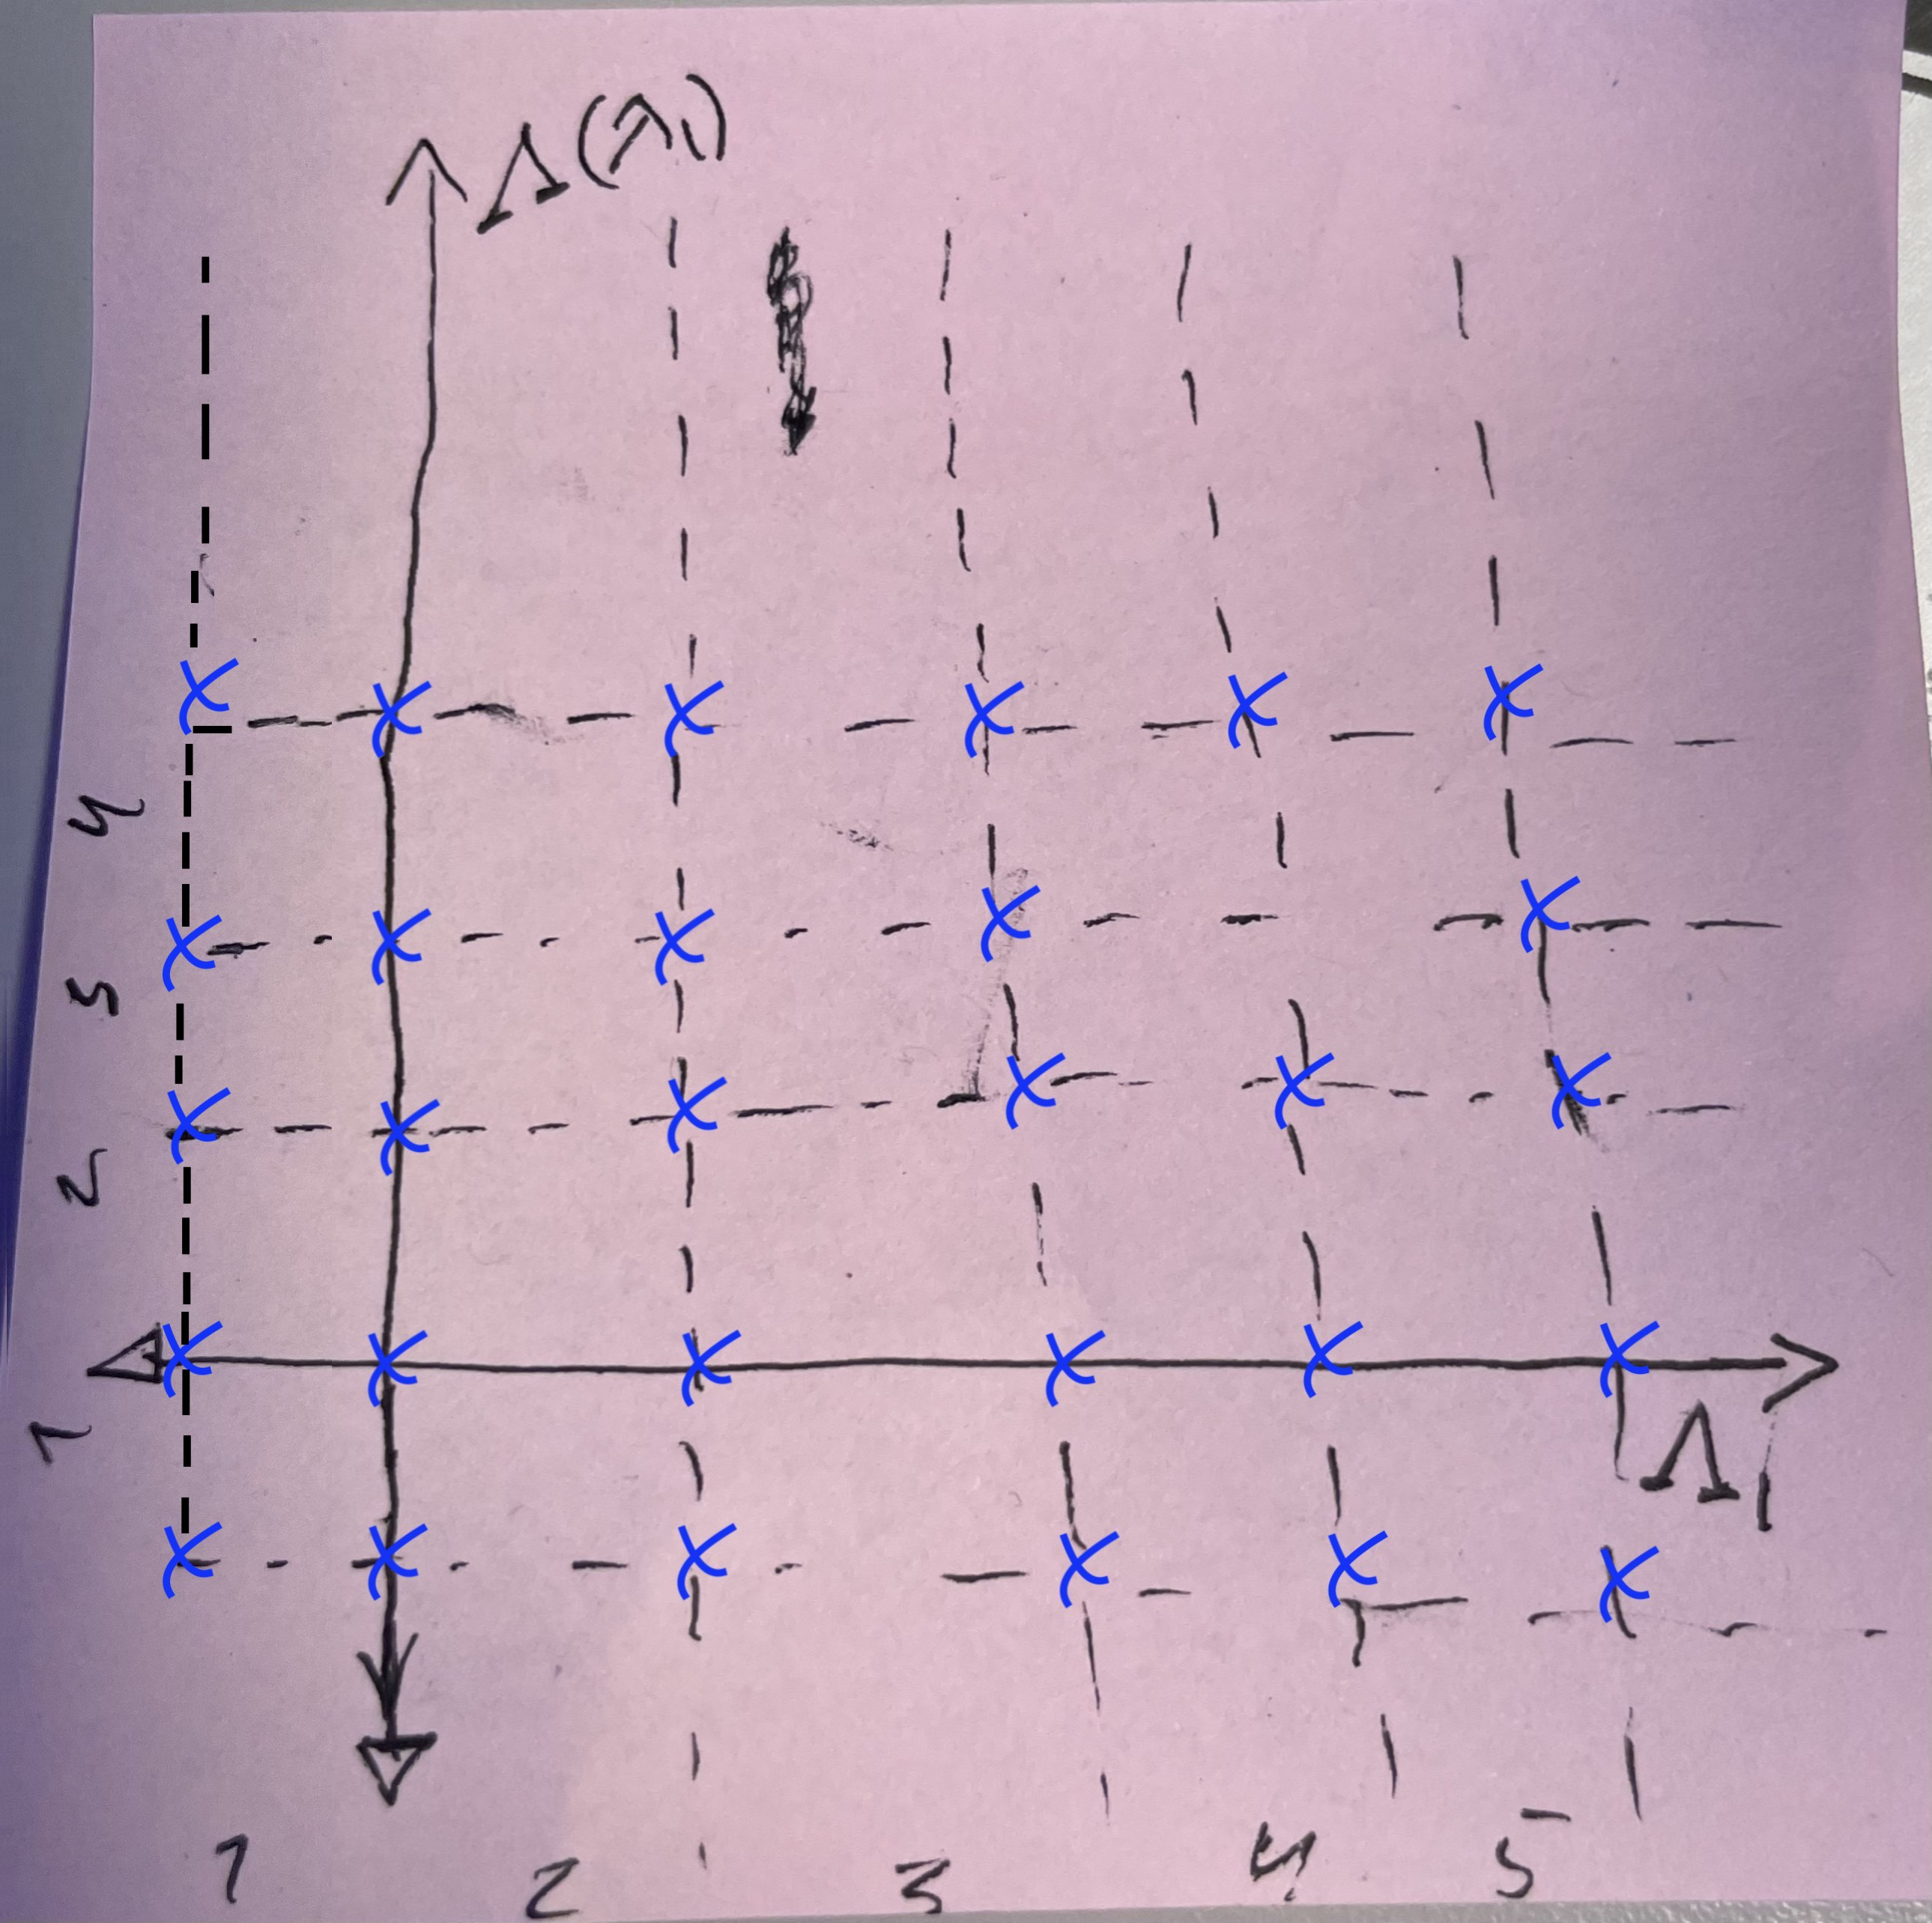
\includegraphics[width=0.9\linewidth]{spec_no_shift.jpg}
        %* Figure 1
        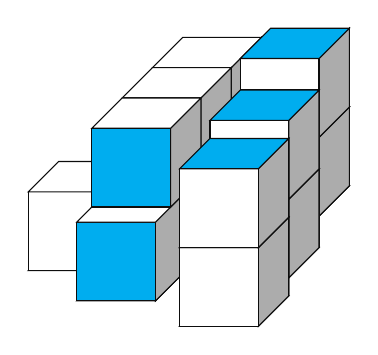
\begin{tikzpicture}[scale=1]
            % Define the tile
            \def\tile{
              % Draw the unit cube
                \draw[black!95] (1,0,0) -- (1,0,1) -- (1,1,1) -- (1,1,0) -- cycle; % left face
                \draw[black!95] (0,0,0) -- (1,0,0) -- (1,0,1) -- (0,0,1) -- cycle; % bottom face
                \draw[black!95] (0,0,0) -- (0,1,0) -- (1,1,0) -- (1,0,0) -- cycle; % back face
                \draw[black!95, fill=gray!65] (1,0,0) -- (1,1,0) -- (1,1,1) -- (1,0,1) -- cycle; % right face
                \draw[black!95, fill=white] (0,0,1) -- (1,0,1) -- (1,1,1) -- (0,1,1) -- cycle; % front face
                \draw[black!95, fill=white](0,1,0) -- (0,1,1) -- (1,1,1) -- (1,1,0) -- cycle; % top face
            }
            
            \def\tiletwo{
                % Draw the unit cube
                    \draw[black!95] (1,0,0) -- (1,0,1) -- (1,1,1) -- (1,1,0) -- cycle; % left face
                    \draw[black!95] (0,0,0) -- (1,0,0) -- (1,0,1) -- (0,0,1) -- cycle; % bottom face
                    \draw[black!95] (0,0,0) -- (0,1,0) -- (1,1,0) -- (1,0,0) -- cycle; % back face
                    \draw[black!95, fill=gray!65] (1,0,0) -- (1,1,0) -- (1,1,1) -- (1,0,1) -- cycle; % right face
                    \draw[black!95, fill=cyan] (0,0,1) -- (1,0,1) -- (1,1,1) -- (0,1,1) -- cycle; % front face
                    \draw[black!95, fill=white](0,1,0) -- (0,1,1) -- (1,1,1) -- (1,1,0) -- cycle; % top face
                }
        
            \def\tilethree{
                % Draw the unit cube
                    \draw[black!95] (1,0,0) -- (1,0,1) -- (1,1,1) -- (1,1,0) -- cycle; % left face
                    \draw[black!95] (0,0,0) -- (1,0,0) -- (1,0,1) -- (0,0,1) -- cycle; % bottom face
                    \draw[black!95] (0,0,0) -- (0,1,0) -- (1,1,0) -- (1,0,0) -- cycle; % back face
                    \draw[black!95, fill=gray!65] (1,0,0) -- (1,1,0) -- (1,1,1) -- (1,0,1) -- cycle; % right face
                    \draw[black!95, fill=white] (0,0,1) -- (1,0,1) -- (1,1,1) -- (0,1,1) -- cycle; % front face
                    \draw[black!95, fill=cyan](0,1,0) -- (0,1,1) -- (1,1,1) -- (1,1,0) -- cycle; % top face
                }
          
            % Draw the tiling pattern
            % For x=0
            \foreach \x in {0}{
               \foreach \y in {0}{
                    \foreach \z in {0}{
                        \pgfmathsetmacro{\shiftX}{\x} % Set horizontal shift
                        \pgfmathsetmacro{\shiftY}{\y} % Set vertical shift
                        \pgfmathsetmacro{\shiftZ}{\z+0.8} % Set vertical shift
                        \begin{scope}[shift={(\shiftX,\shiftY,\shiftZ)}]
                        \tile % Draw the tile
                        \end{scope}
                    }
                }
            }
            % For x=1
            \foreach \x in {1}{
               \foreach \y in {0,1}{
                    \foreach \z in {-1,0,1}{
                        % Here we shift with different z values for each height value 
                        % i.e. Row shift
                        \ifnum\y=0
                            \pgfmathsetmacro{\shiftX}{\x} % Set horizontal shift
                            \pgfmathsetmacro{\shiftY}{\y}
                            \pgfmathsetmacro{\shiftZ}{\z+0.8} % Set vertical shift
                        \fi
                        \ifnum\y=1
                            \pgfmathsetmacro{\shiftX}{\x} % Set horizontal shift
                            \pgfmathsetmacro{\shiftY}{\y}
                            \pgfmathsetmacro{\shiftZ}{\z+0.3} % Set vertical shift
                        \fi
                        \ifnum\y=2
                            \pgfmathsetmacro{\shiftX}{\x} % Set horizontal shift
                            \pgfmathsetmacro{\shiftY}{\y}
                            \pgfmathsetmacro{\shiftZ}{\z-0.5} % Set vertical shift
                        \fi
                        
                        \begin{scope}[shift={(\shiftX,\shiftY,\shiftZ)}]
                        \tiletwo % Draw the tile
                        \end{scope}
                    }
                }
            }
        
            % For x=2
            % The code for this part is a bit divided, thre last columns are here, the one in the very back has same shift as the one in the front
            \foreach \x in {2}{
               \foreach \y in {0,1}{
                    \foreach \z in {-1,0,1}{
                        % Here we shift with different y values for each depth value
                        % i.e. Column shift
                        \ifnum\z=-1
                            \pgfmathsetmacro{\shiftX}{\x} % Set horizontal shift
                            \pgfmathsetmacro{\shiftY}{\y}
                            \pgfmathsetmacro{\shiftZ}{\z} % Set vertical shift
                        \fi
                        \ifnum\z=0
                            \pgfmathsetmacro{\shiftX}{\x} % Set horizontal shift
                            \pgfmathsetmacro{\shiftY}{\y-0.4}
                            \pgfmathsetmacro{\shiftZ}{\z} % Set vertical shift
                        \fi
                        \ifnum\z=1
                            \pgfmathsetmacro{\shiftX}{\x} % Set horizontal shift
                            \pgfmathsetmacro{\shiftY}{\y-0.63}
                            \pgfmathsetmacro{\shiftZ}{\z} % Set vertical shift
                        \fi
                        \begin{scope}[shift={(\shiftX,\shiftY,\shiftZ)}]
                        \tilethree % Draw the tile
                        \end{scope}
                    }
                }
            }
        \end{tikzpicture}
        %* —————————————————
        %\caption{Lattice tiling}
        \label{fig:tiling_six}
    \end{subfigure}
    \caption{Highlighted in cyan are the fully face-sharing edges (left) and squares (right) for $d=2$ and $d=3$, respectively. Observe the two different orientations for the cyan squares.}
    \label{fig:tilings_five_six}
\end{figure}


If the dimension is two, the squares share an edge; if the dimension is three, they share a square. \cref{fig:tilings_five_six} illustrates this. Furthermore, when $d\geq 3$, it is not necessarily true that \emph{all} cubes shared a whole $(n-1)$-dimensional face with one of its neighbors \cite{perronUeberLueckenloseAusfuellung1940}. It is important to emphasize that the \namecref{conj:keller_tiling} does not support the existence of exotic tilings. Instead, it indicates the opposite — rigidity in the tiling of the space. %/ $\R^d$.
However, after being first proven true for $d\leq 6$ by Perron in 1940 \cite{perronModulartigeLueckenloseAusfuellung1940,perronModulartigeLueckenloseAusfuellung1940a}, it has since then gradually been proved false for all $d\geq10$ \cite{lagariasKellerCubetilingConjecture1992} and later all $d\geq8$ \cite{mackeyCubeTilingDimension2002}. The last remaining dimension was finally solved in 2020, where it was proven to be true \cite{brakensiekResolutionKellerConjecture2020}, leading us to a solution in all dimensions for Keller's \namecref{conj:keller_tiling}.%, \cref{conj:keller_tiling}. 

\begin{theorem}
    In all tilings of $\R^d$ by translations of the unit cube, Keller's \namecref{conj:keller_tiling}, \cref{conj:keller_tiling}, is true for all dimensions $d\leq 7$ and false for all $d>7$.
\end{theorem}

%* Longer explanation: "An example of what..."
%While we refer to \cite{brakensiekResolutionKellerConjecture2020} for a comprehensive and detailed exposition on how Keller's conjecture has been reduced and transformed into a graph theoretic problem solved using computer-aided mathematics, to briefly explain the concept and give an example of what these higher-dimensional tilings might look like consider the following: Keller graphs denoted as $G_{d,s}$ consist of vertices given by $\braq{0,1,2,\dots,2s-1}^d$. Here, $d$ is the dimension, and $s$ indicates all the different values a coordinate can take. In this graph, two vertices are considered adjacent if they differ in at least two coordinates, where at least one of these differences must be exactly $s$. Within each graph $G_{d,s}$, we can have cliques of different sizes, but they cannot be larger than $2^d$. However, a clique of size $2^d$ within $G_{d,s}$ would disprove Keller's conjecture for dimensions greater than or equal to that dimension $d$. For dimension $d=8$, a clique of size $2^8=256$ within $G_{8,2}$ is what is depicted in \cref{fig:tiling_seven}. Notably, since $s=2$, this represents the smallest counterexample to Keller's \namecref{conj:keller_tiling}, \cref{conj:keller_tiling}.
\begin{remark}
    Keller also wrote a paper claiming to solve his \namecref{conj:keller_tiling} for $d\leq 6$ \cite{Keller1937}. However, Perron later described Keller's solution for $d=5$ and $d=6$ as \emph{"quite incomprehensible to me"} and \emph{"very sketchy"} in the literal sense of the word \cite{perronUeberLueckenloseAusfuellung1940} \footnote[1]{Perron's origninal description of Keller's solution to his \namecref{conj:keller_tiling}: \emph{— Enthält einen sehr skizzenhaften mir ziemlich unverständlichen Beweis für die Richtigkeit der Kellerchen Vermutung im Falle n=5 unt n=6.}}. Furthermore, what is interesting is the fact that Keller himself later doubted whether his \namecref{conj:keller_tiling} was actually true.
\end{remark}

While we refer to \cite{brakensiekResolutionKellerConjecture2020} for a comprehensive and detailed exposition on how Keller's \namecref{conj:keller_tiling} has been reduced and transformed into a graph theoretic version solved using computer-aided mathematics, to briefly explain the concept consider the following: \emph{Keller graphs} denoted as $G_{d,s}$ consist of \emph{vertices} given by $\braq{0,1,2,\dots,2s-1}^d$. Here, $d$ denotes the dimension, and $s$ denotes the number of \emph{coordinates}. In this graph, two vertices are considered \emph{adjacent} if they differ in at least two coordinates, where at least one of these differences must be exactly $s$. Within each graph $G_{d,s}$, we can have \emph{cliques} of different sizes, but they cannot be larger than $2^d$. A clique is a subgraph with any two adjacent vertices. However, a clique of size $2^d$ within $G_{d,s}$ would disprove Keller's \namecref{conj:keller_tiling} for dimensions greater than or equal to that dimension $d$. This condition is the critical key in resolving the \namecref{conj:keller_tiling} through Keller graphs \cite{corradiCombinatorialApproachKeller1990}. This combinatorial argument was made possible after Hajos reformulated Keller's \namecref{conj:keller_tiling} into an algebraic equivalent, similar to what he did before solving Minkowski's conjecture \cite{lagariasKellerCubetilingConjecture1992,hajosUeberEinfacheUnd1942}. For dimension $d=8$, a clique of size $2^8=256$ within $G_{8,2}$ is what is depicted in \cref{fig:tiling_seven}. Notably, since $s=2$, this also represents the smallest counterexample. %Notably, since $s=2$, this represents the smallest counterexample to Keller's \namecref{conj:keller_tiling}, \cref{conj:keller_tiling}.  %* The coordinate set indicates all the different values a coordinate can take.


% fill=gray!50

\begin{figure}[t!]%h!
    \centering
    \begin{subfigure}{.47\textwidth}
        \centering
        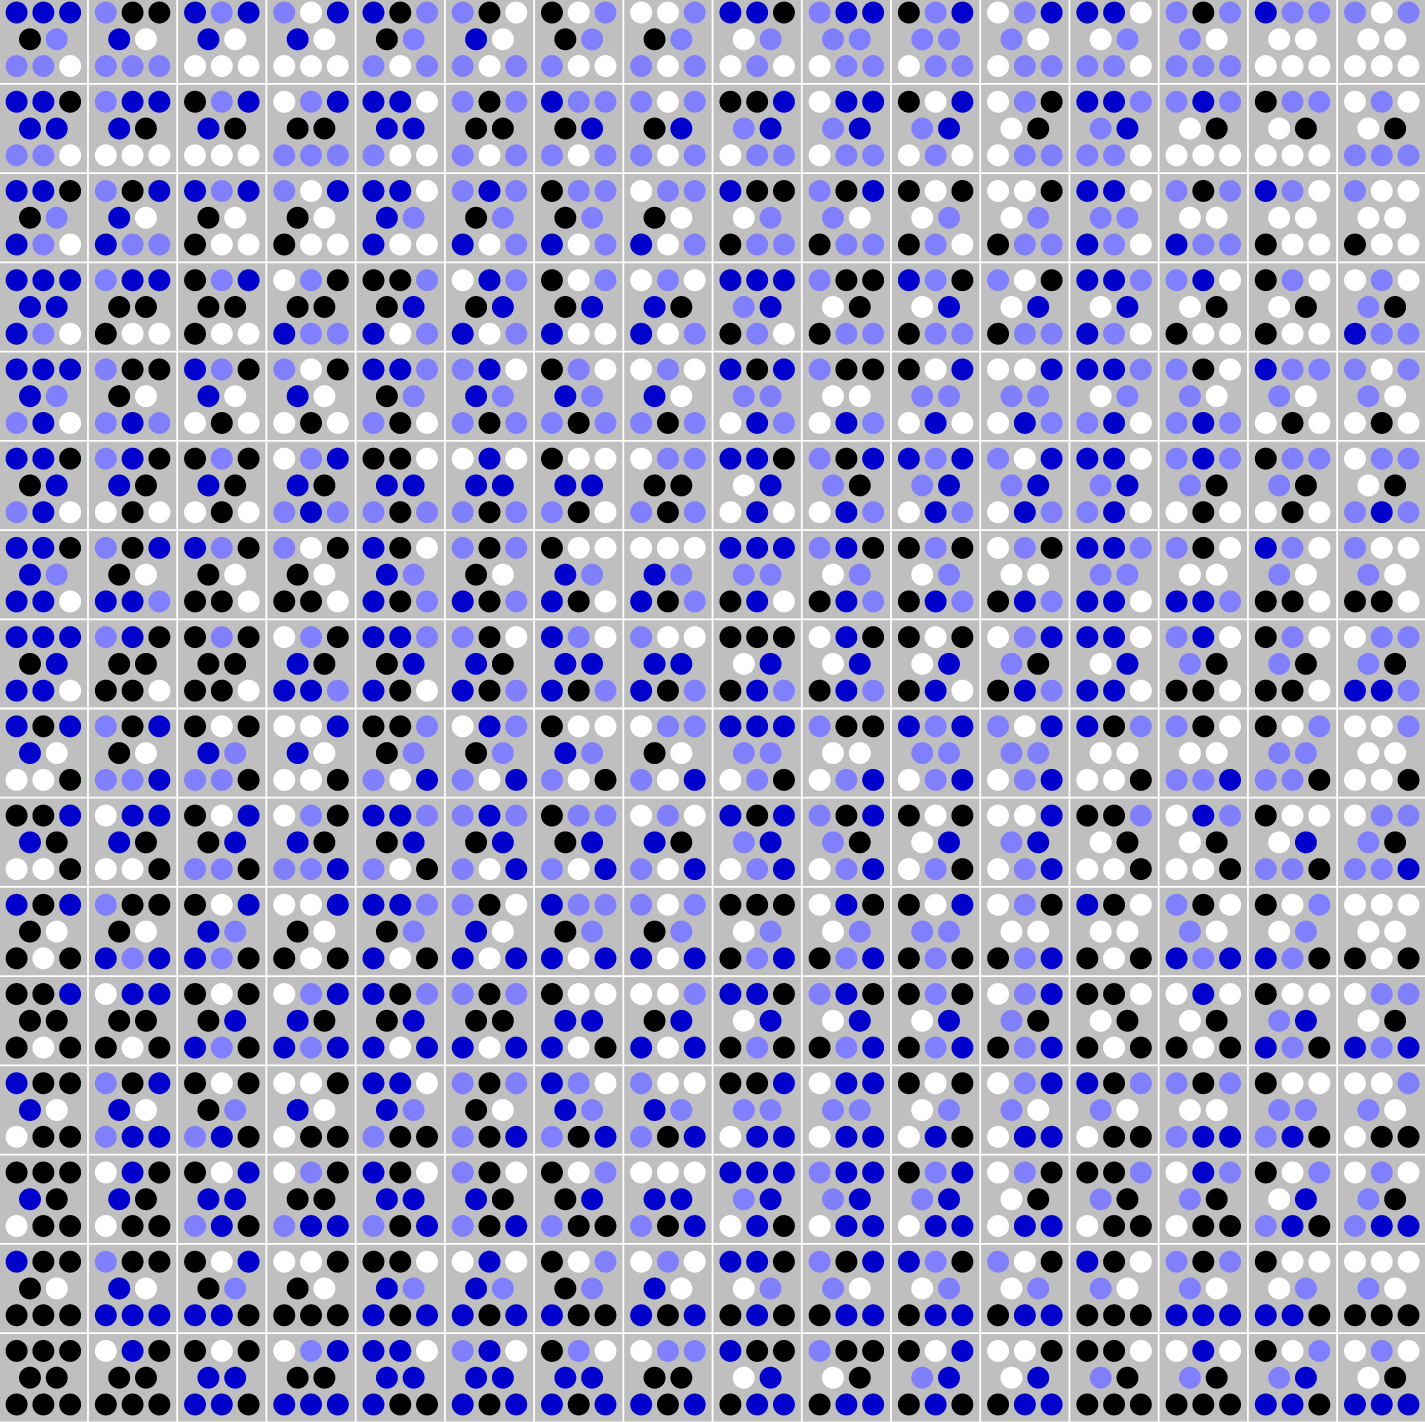
\includegraphics[width=0.9\linewidth]{keller_clique.png}
        %* —————————————————
        \caption{A Keller graph \cite{brakensiekResolutionKellerConjecture2020}}
        \label{fig:tiling_seven}
    \end{subfigure}\quad
    \begin{subfigure}{.47\textwidth}
        \centering
        %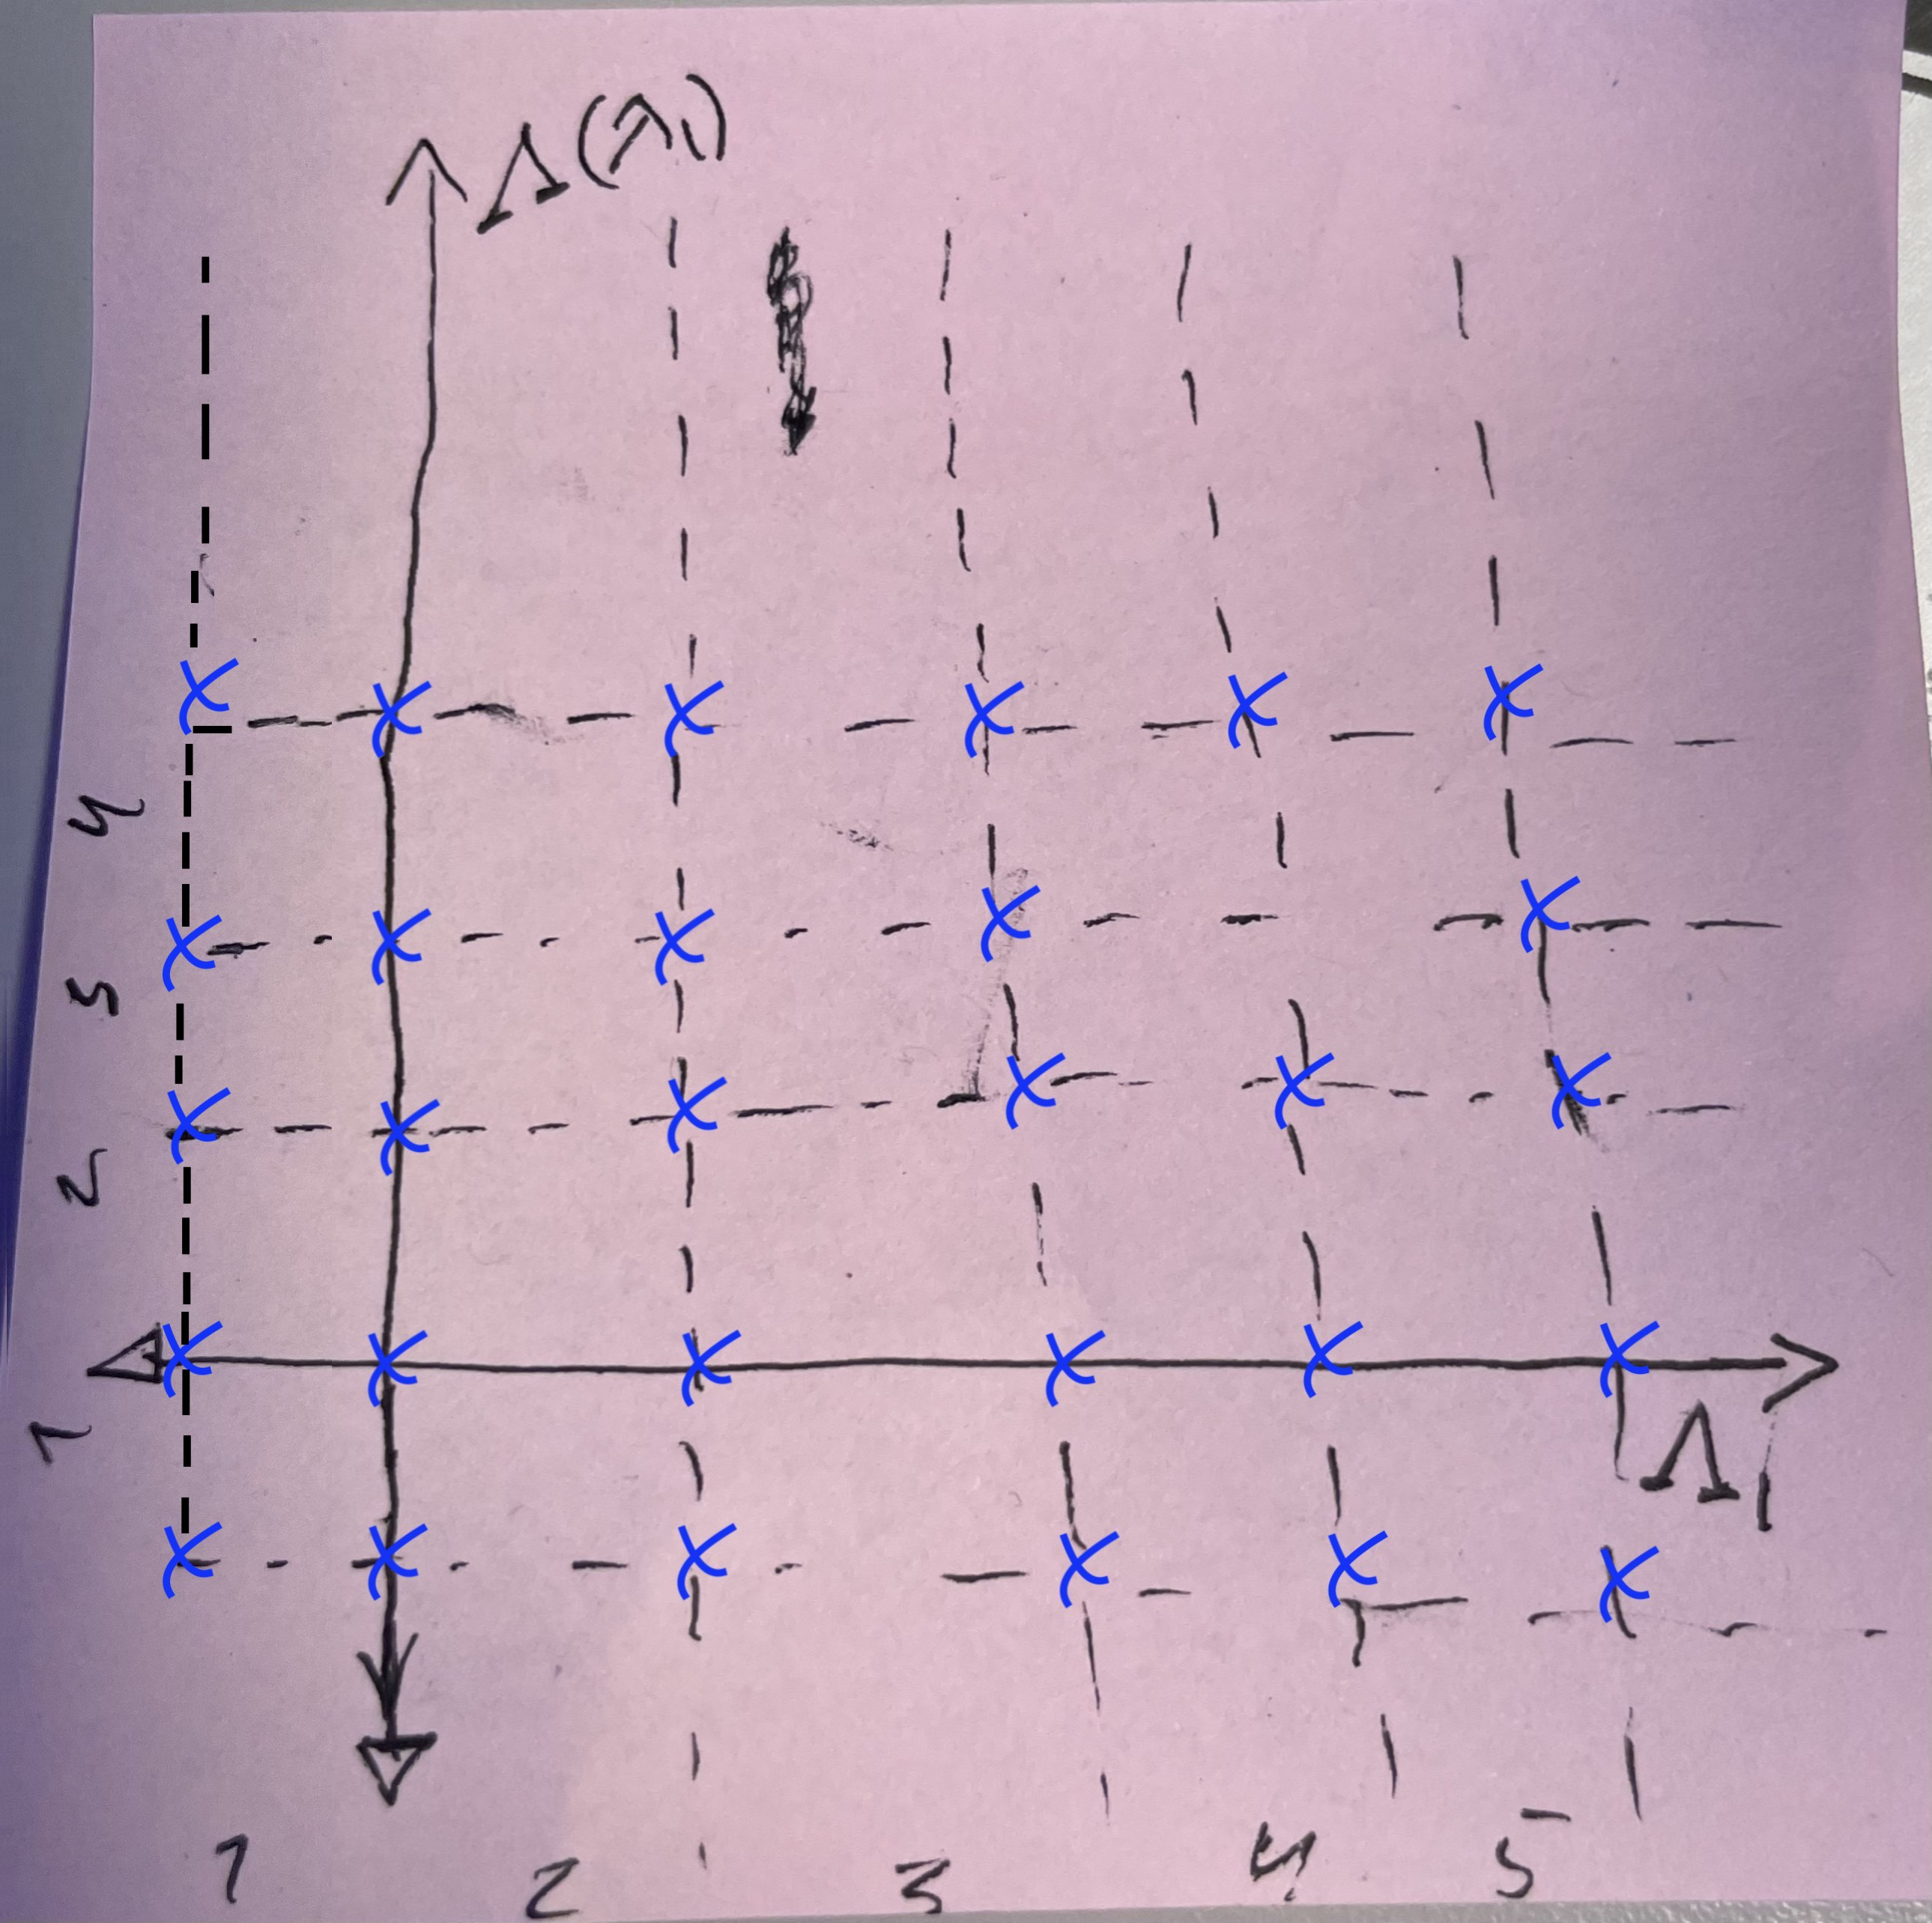
\includegraphics[width=0.9\linewidth]{spec_no_shift.jpg}
        %* Figure 1              
        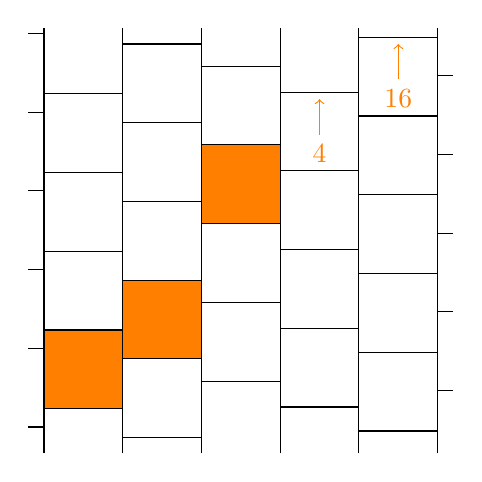
\begin{tikzpicture}[scale=1]
            % Define the tile
            \def\tile{
            % Draw the unit square
            \draw[fill=white] (0,0) rectangle (1,1);
            }
            \def\tiletwo{
            %\draw[fill=gray!65] (0,0) rectangle (1,1);
            \draw[fill=orange] (0,0) rectangle (1,1);
            %\draw[->] (0.5,0) -- (0.5,0.9);  % If arrows from the middle
            }
            % Right border tile
            \def\tileThree{
            %\draw[fill=red] (0,0) rectangle (1,1);  % test tile to se if we got the right one
            \draw[black] (0,1) -- (0+0.2,1);  % Right_top
            \draw[black] (0,0) -- (0+0.2,0);  % Right_bottom
            }
            % Left border tile
            \def\tileFour{
            % If using test square, must change from x=0 to x=1 for the left border markers
            %\draw[fill=red] (0,0) rectangle (1,1);  % test tile to se if we got the right one
            \draw[black] (0,1) -- (0-0.2,1);  % Right_top
            \draw[black] (0,0) -- (0-0.2,0);  % Right_bottom
            }
            
            % Exponential function parameters
            \pgfmathsetmacro{\base}{2} % Base of the exponential function
            \pgfmathsetmacro{\expMinTwo}{exp(-2)}
            \pgfmathsetmacro{\expMinOne}{exp(-1)}
            \pgfmathsetmacro{\expZero}{exp(0)}
            \pgfmathsetmacro{\expOne}{exp(1)}
            \pgfmathsetmacro{\expTwo}{exp(2)}
            \pgfmathsetmacro{\expThree}{exp(3)}
            \pgfmathsetmacro{\expFour}{exp(4)}

            % Shift list
            \def\BetaMinOne{\expMinOne}
            \def\BetaZero{\expZero}
            \def\BetaOne{\expOne}
            \def\BetaTwo{\expTwo}
            \def\BetaThree{\expThree}
            \def\BetaFour{\expFour}

            % Left border markers
            \foreach \x in {0}{
                \foreach \y in {0,1,2,3,4}{
                    \pgfmathsetmacro{\shiftX}{\x}
                    \pgfmathsetmacro{\shiftY}{\y + \expMinTwo}
                    \pgfmathsetmacro{\shiftSingle}{\expMinTwo}
                    
                    % Drawing the rest of the middle cubes
                    \begin{scope}[shift={(\shiftX,\shiftY)}]
                        \tileFour
                    \end{scope}
        }}
            % Right border markers
            \foreach \x in {5}{
                \foreach \y in {-54,...,-51}{
                    \pgfmathsetmacro{\shiftX}{\x}
                    \pgfmathsetmacro{\shiftY}{\y + \BetaFour}
                    \pgfmathsetmacro{\shiftSingle}{\BetaFour}
                    % Drawing the rest of the middle cubes
                    \begin{scope}[shift={(\shiftX,\shiftY)}]
                        \tileThree
                    \end{scope}
                    
        }}


            % Draw the tiling pattern Latter part
            \foreach \x in {1}{
                \foreach \y in {-1,...,3}{
                    \pgfmathsetmacro{\shiftX}{\x}
                    \pgfmathsetmacro{\shiftY}{\y + \BetaZero}
                    \pgfmathsetmacro{\shiftSingle}{\BetaZero}
                    % Drawing the rest of the middle cubes
                    \begin{scope}[shift={(\shiftX,\shiftY)}]
                        \tile
                    \end{scope}
                    % No need for orange cubes as they would be outside
                }}
            \foreach \x in {2}{
                \foreach \y in {-2,...,1}{
                    \pgfmathsetmacro{\shiftX}{\x} 
                    \pgfmathsetmacro{\shiftY}{\y + \BetaOne} 
                    \pgfmathsetmacro{\shiftSingle}{0+\BetaOne}
                    % Drawing the rest of the middle cubes
                    \begin{scope}[shift={(\shiftX,\shiftY)}]
                        \tile
                    \end{scope}
                    % No need for orange cubes as they would be outside
                }}
            \foreach \x in {3}{
                \foreach \y in {-7,...,-4}{
                    \pgfmathsetmacro{\shiftX}{\x}
                    \pgfmathsetmacro{\shiftY}{\y + \BetaTwo}
                    \pgfmathsetmacro{\shiftSingle}{\BetaTwo}
                    % Drawing the rest of the middle cubes
                    \begin{scope}[shift={(\shiftX,\shiftY)}]
                        \tile
                    \end{scope}
                    % No need for orange cubes as they would be outside
                    % REMEMBER that we have shifted the entirety of what is plotted from this column, 
                    % our grid is still x: -1,...,5 and   y: 0,...,4 i.e., The leftmost markers!!                  
                    \ifnum\y=-4
                        \draw[->, orange] (\x+0.5,3.85) node[below] {$4$} -- (\x+0.5,4.3);
                    \fi
                }}
                \foreach \x in {4}{
                    \foreach \y in {-20,...,-16}{
                    \pgfmathsetmacro{\shiftX}{\x}
                    \pgfmathsetmacro{\shiftY}{\y + \BetaThree}
                    \pgfmathsetmacro{\shiftSingle}{\BetaThree}
                    % Drawing the rest of the middle cubes
                    \begin{scope}[shift={(\shiftX,\shiftY)}]
                        \tile
                    \end{scope}
                    % No need for orange cubes as they would be outside
                    % REMEMBER that we have shifted the entirety of what is plotted from this column, 
                    % our grid is still x: -1,...,5 and   y: 0,...,4 i.e., The leftmost markers!!               
                    \ifnum\y=-16
                        \draw[->, orange] (\x+0.5,4.55) node[below] {$16$} -- (\x+0.5,5);
                    \fi
                }}
                
            % Draw the tiling pattern
            \foreach \x in {0}{
                \foreach \y in {0,1,2,3}{
                    \pgfmathsetmacro{\shiftX}{\x}
                    \pgfmathsetmacro{\shiftY}{\y + \BetaMinOne}
                    \pgfmathsetmacro{\shiftSingle}{0+\BetaMinOne}
                    % Drawing the rest of the middle cubes
                    \begin{scope}[shift={(\shiftX,\shiftY)}]
                        \tile
                    \end{scope}
                }  
            }
            
            % Orange cube overlay
            \foreach \x in {0,1,2}{
                \foreach \y in {0,1,2,3}{
                    \ifnum\x=0
                        \pgfmathsetmacro{\shiftX}{\x}
                        \pgfmathsetmacro{\shiftY}{\y + \BetaMinOne}
                        \pgfmathsetmacro{\shiftSingle}{0+\BetaMinOne}
                    \fi
                    \ifnum\x=1
                        \pgfmathsetmacro{\shiftX}{\x}
                        \pgfmathsetmacro{\shiftY}{\y + \BetaZero}
                        \pgfmathsetmacro{\shiftSingle}{0+\BetaZero}
                    \fi
                    \ifnum\x=2
                        \pgfmathsetmacro{\shiftX}{\x}
                        \pgfmathsetmacro{\shiftY}{\y + \BetaOne}
                        \pgfmathsetmacro{\shiftSingle}{0+\BetaOne}
                    \fi
                    % Drawing a new line of shifted colored cubes on top at the first row
                    \ifnum\y=0
                        \begin{scope}[shift={(\shiftX,\shiftY)}]
                            \tiletwo
                        \end{scope}
                    \fi
        }}
            % get the outline grid 
            % Whole black lines
            \foreach \x in {0,1,2,3,4,5}{
                \draw (\x,0-0.2) -- (\x,5+0.2);  % Shift only in the vertical direction, therefore only one line
            }
        \end{tikzpicture}
        %* —————————————————
        \caption{Non-periodic tiling of unit cubes}
        \label{fig:tiling_eight}
    \end{subfigure}
    \caption{Illustrated in \cref{fig:tiling_seven} is a clique of size $2^8=256$ in the Keller graph of $G_{8,2}$, which disproves Keller's conjecture for $d\geq8$. Each grey square of $8$ dots represents a vertex, and each dot inside the square represents a coordinate. The coordinate set in the Keller graph of $G_{8,2}$ is $\braq{0,1,2,3}$, where the colors black, dark blue, white, or light blue respectively represents each of the possible coordinate values. Observe that for the vertices to be adjacent, it is enough for any two vertices to have a complimentary dot, which means either black versus white or dark blue versus light blue; \textsc{and} at least one dot of a different color as a different color represents a different coordinate. Illustrated in \cref{fig:tiling_eight} is a non-periodic tiling of $\R^2$ where the $n$'th column of unit cubes is shifted in the vertical direction by the value of $e^n$, for all $n\in\Z$. The arrow with an orange number indicates the number of unit squares from the arrow to the orange-colored unit square. If this were a lattice tiling, all orange-colored squares would be on the same horizontal line. The lines of the $-2$'th and $4$'th columns of unit cubes can be observed at the left and right edges, respectively.}
    \label{fig:tilings_seven_eight}
\end{figure}

% In addition to the tilings related to Keller's \namecref{conj:keller_tiling}, \emph{periodicity} is another essential concept. A monohedral tiling is \emph{non-periodic} if it admits no period parallelograms \cite{penrosePentaplexityClassNonPeriodic1979}, and \emph{vice versa}. In our case, this intuitively means that if we know the arrangement of the tile with respect to its vertices and edges within a parallelogram, then we can construct the entire tiling by repeating this arrangement. That is, repeating the parallelogram, not the tile. We refer to \cite[p.29-30]{grunbaumTilingsPatterns1987} for an in-depth explanation with great images. Nevertheless, if our tile exclusively tiles non-periodically, then we say it is \emph{aperiodic}. That is, \emph{every} tiling possible with the tile is non-periodic and must necessarily be so \cite[p. 520]{grunbaumTilingsPatterns1987}. It is critical to make the distinction here that in this context, it is the \emph{tile} that is considered to be aperiodic and not the tiling itself. An \emph{aperiodic tiling}, on the other hand, instead means a complete absence of a period (parallelogram \SigridChange{Correct? with this parallelogram addition?}) in \emph{all} coordinates. And as we informally defined above, if there is a period in at least \emph{one} of the coordinates, it is non-periodic tiling; if there is a period in all directions, then it is a periodic tiling\footnote[1]{These terms have been confusing in the papers studied, which is why we stress these distinctions.}. 
In addition to the tilings related to Keller's \namecref{conj:keller_tiling}, the concept of \emph{periodicity} is essential. A monohedral tiling is considered \emph{non-periodic} if it does not allow any period parallelograms \cite{penrosePentaplexityClassNonPeriodic1979}, and \emph{vice versa}. Essentially, this means that if we know the arrangement of the tiles with respect to their vertices and edges within a parallelogram, we can construct the entire tiling by repeating this arrangement. It is important to note that we repeat the parallelogram, not the tile itself. For a more detailed explanation accompanied by illustrative figures, please refer to \cite[p.29-30,147-149]{grunbaumTilingsPatterns1987}. 

Furthermore, if a tile exclusively allows for non-periodic tilings, we consider it to be \emph{aperiodic}. This indicates that \emph{every} tiling possible with the tile is non-periodic and must necessarily be so \cite[p. 520]{grunbaumTilingsPatterns1987}. It is crucial to establish a clear distinction in this context: the term 'aperiodic' specifically relates to the characteristics of the \emph{tile} itself rather than the overall tiling. In contrast, when we refer to an \emph{aperiodic tiling}, we precisely describe a tiling configuration that completely lacks any period (parallelogram \SigridChange{Correct? with this parallelogram addition?}) across \emph{all} coordinates/directions. This statement is stronger than a non-periodic tiling, requiring only at least \emph{one} coordinates/directions with no period. Similarly note, if there is a period in \emph{all} coordinates/directions, then it is a periodic tiling\footnote[1]{These terms have been confusing for the author in the papers studied (cite??????), which is why we stress these distinctions.} CITE(must find citation for this informal definition?) The best definition I have found is the cover of chapter 10 (p. 519 book, or search for "aperiodic tiling." I will check for an informal definition in Aperiodic Order
Volume 1: A Mathematical Invitation. )

In higher dimensions, the unit cube can also tile non-periodically. Two simple examples are illustrated in \cref{fig:single_shift_horizontal_tiling,fig:single_shift_vertical_tiling}. Try creating a single parallelogram that can be used to tile the entire plane, and one will quickly see that this is impossible. However, one can consider them to be \emph{half-periodic}, in the sense that they do not admit a vertical or horizontal period, respectively, but do allow for a period in the same direction as the shift. That is a horizontal and vertical period, respectively \cite{kolountzakisTilingsTranslation2010}. Another simple example of a non-periodic tiling in dimension $2$ is to shift the $n$'th column of unit cubes in the vertical (or horizontal) direction with $e^n$, for all $n\in\Z$ \cite{liuUniformityNonUniformGabor2003}. This is illustrated in \cref{fig:tiling_eight}. These examples are significant because it shows that the unit cube can tile non-periodically in all $d\geq 2$. However, as the unit cube can always be organized into a lattice and hence tile periodically, it is not an aperiodic tile. However, surprisingly, the unit cube can also tile aperiodically in all $d\geq 3$, which will be a topic for \cref{sec:aperi_cube}. 

It is precisely the higher dimensional tilings that are either non-periodic or counterexample Keller's \namecref{conj:keller_tiling} that we intuitively define to be the exotic and counterintuitive tilings.

%* ———————————————————————————— Tilings ——————————————————
%* Here, in the definitions of tiling, we allow the distinct translations of the domain to overlap on sets of measure zero rather than the traditional condition of empty overlap.
%- Now, in defining a tiling more formally, one possible approach is to define it as a non-overlapping covering of the space.
Now, we endeavor to establish a more rigorous definition of tiling. One possible approach is to define it as a non-overlapping covering of the space. By this, we mean that a subset $\Omega \subset \R^d$ of non-zero measure is a tile, and a set $\Lambda \subset \R^d$ is a tiling set if they satisfy both of the following conditions. First, $\Omega+\lambda$ for $\lambda \in \Lambda$ must cover $\R^d$ up to measure zero. Secondly, all intersections $(\Omega+\lambda) \cap (\Omega+\lambda')$ of distinct elements $\lambda,\lambda' \in \Lambda$ must have measure zero. Note that $\Omega+\lambda$ denotes the translate of $\Omega$ by the vector $\lambda$. However, instead of the more intuitive geometric definition, we use the following as our working \namecref{def:tiling} in terms of indicator functions \cite{kolountzakisTilingsTranslation2010,kolountzakisStructureTilingsLine1996}.  % - However, instead of the more intuitive geometric definition, we use the following as our working definition in terms of indicator functions \cite{kolountzakisTilingsTranslation2010,kolountzakisStructureTilingsLine1996}.
% - More formally/Nevertheless, tilings can also be expressed using indicator functions as follows \cite{kolountzakisTilingsTranslation2010}. \SigridChange{/} We will, however, define tilings in terms of indicator functions as follows \cite{kolountzakisTilingsTranslation2010} \cite{kolountzakisStructureTilingsLine1996}.
% - Rather than defining tiling in terms of a non-overlapping covering of the space, we will instead define tiling by the indicator function, using little of our geometric intuition \cite{kolountzakisTilingsTranslation2010} \cite{kolountzakisStudyTranslationalTiling2003}. 
\begin{definition}[Tiling set]\label{def:tiling}
    Let $\Omega \subset \R^d$ be a subset with non-zero measure, and consider a discrete set $\Lambda \subset \R^d$. If
    \begin{equation}\label{eq:tiling_set}
        \sum_{\lambda \in \Lambda} \indicator{\Omega}{x-\lambda} = 1, \quad a.e. \text{\space\space} x \in \R^d.
    \end{equation}
    then $\Omega$ is called a \emph{tile}, and $\Lambda$ is called a \emph{tiling set} for $\Omega$. We say that $(\Omega, \Lambda)$ is a \emph{tiling pair}.
\end{definition}
\begin{remark}
    We can also say that $\Omega$ \emph{tiles $\R^d$ by translation}, or that $\Omega$ is a \emph{tiling} of $\R^d$. 
\end{remark}
\begin{remark}
    Additionally, one can define tilings more generally. By this, we mean that in place of the indicator function, we can have a non-negative, integrable function $f$. Other than allowing for any other constant value than $1$, the definition is the same. The reader is referred to \cite{kolountzakisTilingsTranslation2010,kolountzakisStructureTilingsLine1996} for more details on this topic.
\end{remark}
% Direct in text:
% In other words, we can also say that $\Omega$ \emph{tiles $\R^d$ by translation}, or that $\Omega$ is a \emph{tiling} of $\R^d$. Additionally, one can define tilings more generally. By this, we mean that in place of the indicator function, we can have a non-negative, integrable function $f$. Other than allowing for any other constant value than $1$, the definition is the same. Note that we still require the same constant value almost everywhere. The reader is referred to \cite{kolountzakisTilingsTranslation2010} for more details on this topic.
\end{document}